\chapter{CHÍNH SÁCH CỦA
  CHÍNH PHỦ}

\section{ Sản phẩm X có hàm cung và hàm cầu là:}
$Q_S = P - 20 $  $ Q_D = 120 - P$ \\
(P tính bằng nghìn đồng/tấn, Q tính bằng triệu tấn)

\begin{enumerate}[a.]
    \item Xác định giá và sản lượng cân bằng trên thị trường.

          $Q_S = P - 20 = Q_D = 120 - P$
          $\Rightarrow 2P = 140 \Rightarrow P = 70, Q = 50$

    \item Chính phủ áp đặt mức giá trần $P_C= 50$ nghìn đồng/tấn thì điều gì xảy ra trên thị trường?
          Tại sao? Tính CS, PS tại mức giá trần này.



          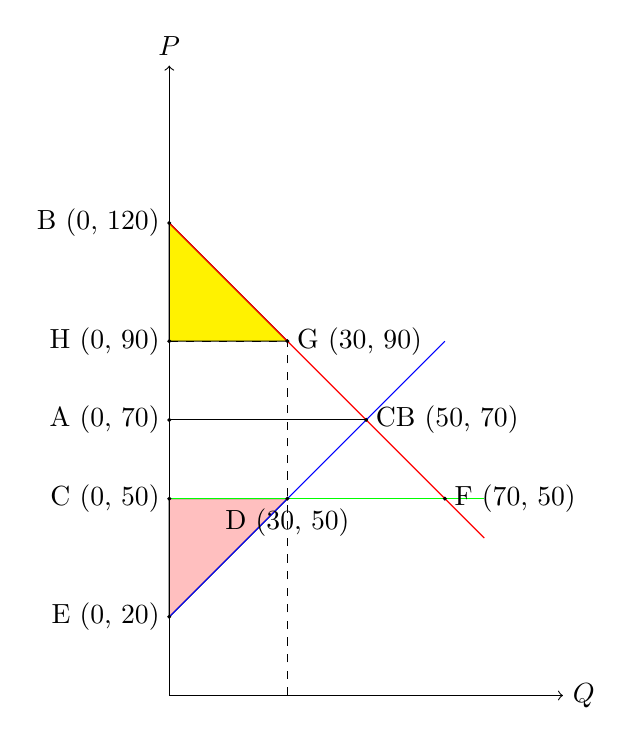
\begin{tikzpicture}
              \draw [->] (0,0) -- (5,0)node[right] {$Q$};
              \draw [->] (0,0) -- (0,8)node[above] {$P$};

              \filldraw[fill=yellow, scale = 0.05] (0,90) -- (30,90) -- (0, 120) -- cycle;
              %\filldraw[fill=green, scale = 0.5] (0,3) -- (7,3) -- (4, 0) -- (0, 0) -- cycle;
              \filldraw[fill=pink, scale = 0.05] (0,50) --  (30, 50) -- (0, 20) -- cycle;

              \draw[scale = 0.05, domain=0:80, smooth, variable=\x, color=red]
              plot ({\x}, {120 - \x});
              \draw[scale = 0.05, domain=0:70, smooth, variable=\x, color=blue]
              plot ({\x}, {\x + 20});

              \draw [-, scale = 0.05, color=green] (0,50) -- (80,50);
              \draw [-, scale = 0.05, color=black] (0,70) -- (50,70);
              \draw [dashed, scale = 0.05, color=black] (30,0) -- (30,90);
              \draw [dashed, scale = 0.05, color=black] (0,90) -- (30,90);

              \filldraw[scale = 0.05, color=black] (50, 70)          circle (10pt) node[anchor=west]{CB (50, 70)};
              \filldraw[scale = 0.05, color=black] (0, 70)          circle (10pt) node[anchor=east]{A (0, 70)};
              \filldraw[scale = 0.05, color=black] (0, 120)          circle (10pt) node[anchor=east]{B (0, 120)};

              \filldraw[scale = 0.05, color=black] (0, 50)          circle (10pt) node[anchor=east]{C (0, 50)};

              \filldraw[scale = 0.05, color=black] (30, 50)          circle (10pt) node[anchor=north]{D (30, 50)};

              \filldraw[scale = 0.05, color=black] (70, 50)          circle (10pt) node[anchor=west]{F (70, 50)};

              \filldraw[scale = 0.05, color=black] (0, 20)          circle (10pt) node[anchor=east]{E (0, 20)};
              \filldraw[scale = 0.05, color=black] (30, 90)          circle (10pt) node[anchor=west]{G (30, 90)};
              \filldraw[scale = 0.05, color=black] (0, 90)          circle (10pt) node[anchor=east]{H (0, 90)};

          \end{tikzpicture}

          tình trạng hiện tại là dư cầu \\
          CS = diện tích BHG = (120 - 90) * 30 / 2 = 450 , \\
          PS = diện tích CDE = (50 - 20) * 30 / 2 = 450


    \item Nếu chính phủ áp đặt giá sàn $P_f = 80$ nghìn đồng/tấn thì điều gì xảy ra trên thị trường?
          Tại sao? Tính CS, PS tại mức giá sàn này.
          Để cho mức giá sàn có hiệu lực thì nhà nước phải làm gì? Số tiền chính phủ phải chi ra
          là bao nhiêu?

          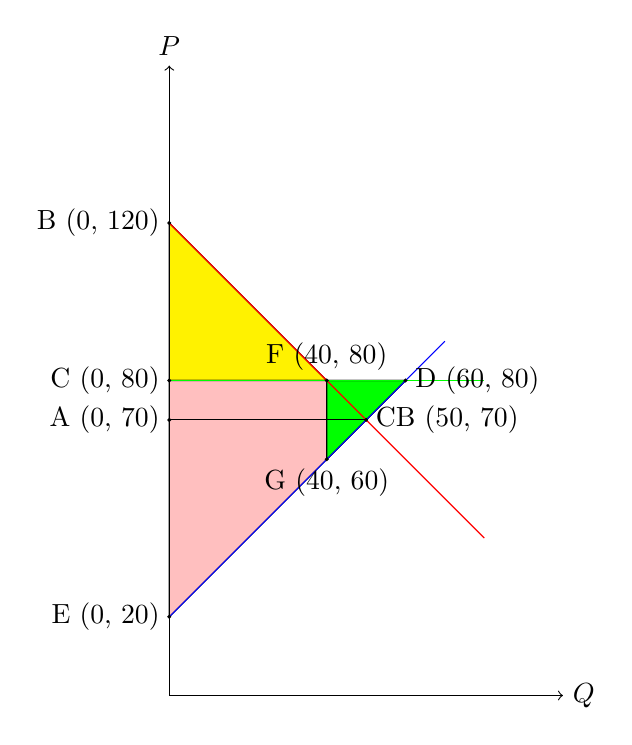
\begin{tikzpicture}
              \draw [->] (0,0) -- (5,0)node[right] {$Q$};
              \draw [->] (0,0) -- (0,8)node[above] {$P$};

              \filldraw[fill=yellow, scale = 0.05] (0,80) -- (40,80) -- (0, 120) -- cycle;
              \filldraw[fill=pink, scale = 0.05] (0,80) --  (60, 80) -- (0, 20) -- cycle;
              \filldraw[fill=green, scale = 0.05] (40,80) -- (60, 80) -- (40, 60) -- cycle;

              \draw[scale = 0.05, domain=0:80, smooth, variable=\x, color=red]
              plot ({\x}, {120 - \x});
              \draw[scale = 0.05, domain=0:70, smooth, variable=\x, color=blue]
              plot ({\x}, {\x + 20});

              \draw [-, scale = 0.05, color=green] (0,80) -- (80,80);
              \draw [-, scale = 0.05, color=black] (0,70) -- (50,70);

              \filldraw[scale = 0.05, color=black] (50, 70)          circle (10pt) node[anchor=west]{CB (50, 70)};
              \filldraw[scale = 0.05, color=black] (0, 70)          circle (10pt) node[anchor=east]{A (0, 70)};
              \filldraw[scale = 0.05, color=black] (0, 120)          circle (10pt) node[anchor=east]{B (0, 120)};

              \filldraw[scale = 0.05, color=black] (0, 80)          circle (10pt) node[anchor=east]{C (0, 80)};

              \filldraw[scale = 0.05, color=black] (60, 80)          circle (10pt) node[anchor=west]{D (60, 80)};

              \filldraw[scale = 0.05, color=black] (40, 80)          circle (10pt) node[anchor=south]{F (40, 80)};

              \filldraw[scale = 0.05, color=black] (0, 20)          circle (10pt) node[anchor=east]{E (0, 20)};

              \filldraw[scale = 0.05, color=black] (40, 60)          circle (10pt) node[anchor=north]{G (40, 60)};

          \end{tikzpicture}

          tình trạng hiện tại là dư cung \\
          CS = diện tích BCF = (120 - 80) * 40 / 2 = 800 , \\
          PS = diện tích CDE = (80 - 20) * 60 / 2 = 1800 \\
          Để cho mức giá sàn có hiệu lực thì nhà nước phải làm gì? Số tiền chính phủ phải chi ra
          là bao nhiêu? \\
          để áp đặt mức giá này thì chính phủ cần thu mua số lượng hàng dư thừa
          lượng tiền bỏ ra là diện tích FGD = (60 - 40) * (80 - 60) / 2 = 200

\end{enumerate}

\section{ Thị trường thịt gà có phương trình hàm cung và cầu như sau:}
$Q_S = 2,5P - 12,5$  $Q_D = 100 - 2P$ \\
(P tính bằng nghìn đồng/kg, Q tính bằng triệu kg)

\begin{enumerate}[a.]
  \item Xác định giá và sản lượng cân bằng trên thị trường.

        $Q_S = 2.5P - 12.5 = Q_D = 100 -   2P$
        $\Rightarrow 4.5P = 112.5 \Rightarrow P = 25, Q = 50$

  \item Nếu chính phủ đánh thuế 1,8 nghìn đồng/1kg vào người bán thì giá mới sẽ là bao nhiêu?
        Giá người bán, người mua phải chịu là bao nhiêu? Thuế mà người mua và người bán phải
        nộp là bao nhiêu?

        ta lưu ý tại hình 6.5 slide 5: Đường cung dịch chuyển lên trên 1 khoảng đúng  bằng mức thuế t

        $Q_S = 2.5P - 12.5 \Rightarrow P = Q_S / 2.5 + 5$ \\
        $P = Q_S / 2.5 + 5 + 1.8 = Q_S / 2.5 + 6.8$\\
        điểm cân bằng mới sẽ tính như sau \\
        $P = Q_S / 2.5 + 6.8 \Rightarrow Q_S = 2.5P - 17 = Q_D = 100 - 2P$\\
        $4.5P = 117 \Rightarrow P = 26, Q = 48$ giá mới là 26


        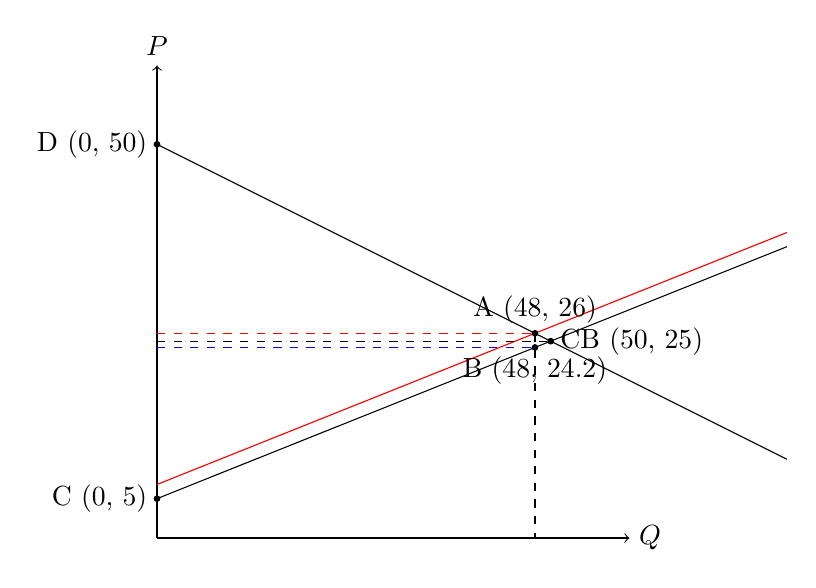
\begin{tikzpicture}
          \draw [->] (0,0) -- (6,0)node[right] {$Q$};
          \draw [->] (0,0) -- (0,6)node[above] {$P$};

          \draw[scale = 0.1, domain=0:80, smooth, variable=\x, color=black]
          plot ({\x}, {50 - \x / 2});
          \draw[scale = 0.1, domain=0:80, smooth, variable=\x, color=black]
          plot ({\x}, {\x / 2.5 + 5});
          \draw[scale = 0.1, domain=0:80, smooth, variable=\x, color=red]
          plot ({\x}, {\x / 2.5 + 6.8});


          \draw [dashed, scale = 0.1, color=black] (0,25) -- (50,25);
          \draw [dashed, scale = 0.1, color=black] (48, 26) -- (48, 0);
          \draw [dashed, scale = 0.1, color=red] (0, 26) -- (48, 26);
          \draw [dashed, scale = 0.1, color=blue] (0, 24.2) -- (48, 24.2);


          \filldraw[scale = 0.1, color=black] (50, 25) circle (10pt) node[anchor=west]{CB (50, 25)};
          \filldraw[scale = 0.1, color=black] (48, 26)  circle (10pt) node[anchor=south]{A (48, 26)};
          \filldraw[scale = 0.1, color=black] (48, 24.2)  circle (10pt) node[anchor=north]{B (48, 24.2)};
          \filldraw[scale = 0.1, color=black] (0, 5)  circle (10pt) node[anchor=east]{C (0, 5)};
          \filldraw[scale = 0.1, color=black] (0, 50)  circle (10pt) node[anchor=east]{D (0, 50)};          

        \end{tikzpicture}

        Giá người bán chịu là giao của đường cung và đường song song với trục tung và đi qua điểm cân bằng mới tại đó Q = 48 do đó P = 24.2,\\
        giá người người mua phải chịu là giá tại điểm cân bằng mới P = 26 \\
        Thuế mà người mua là khoảng cách giữa giá mua và giá cân bằng trước thuế = 26 - 25 = 1\\
        thuế người bán phải nộp là khoảng cách giữa giá thực bán và giá cân bằng trước thuế = 25 - 24.2 = 0.8

  \item Vẽ đồ thị minh họa tác động của thuế ở câu b? Tính CS, PS, TS và phần mất không (DWL)
        của việc đánh thuế này?

        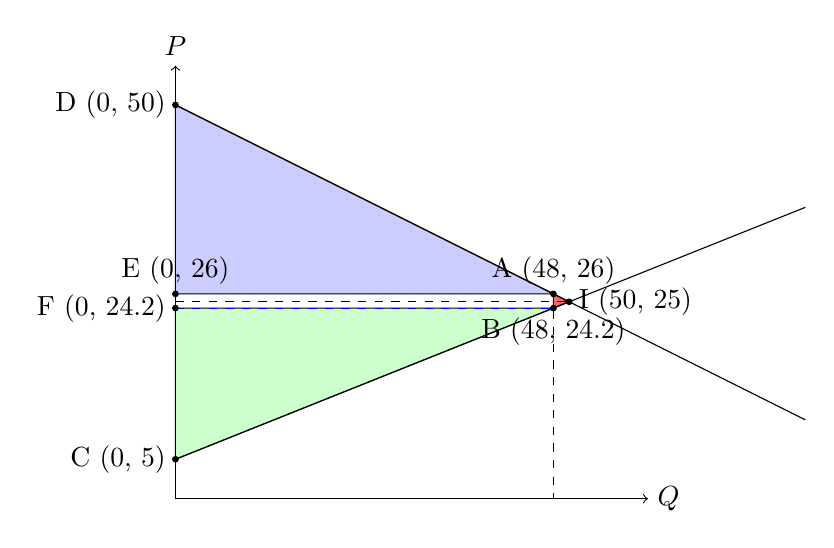
\begin{tikzpicture}
          \draw [->] (0,0) -- (6,0)node[right] {$Q$};
          \draw [->] (0,0) -- (0,5.5)node[above] {$P$};

          \filldraw[fill=blue!20, scale = 0.1] (0,50) -- (48,26) -- (0, 26) -- cycle;
          \filldraw[fill=green!20, scale = 0.1] (0,24.2) -- (48,24.2) -- (0, 5) -- cycle;
          \filldraw[fill=red!60, scale = 0.1] (50,25) -- (48,26) -- (48, 24.2) -- cycle;

          \draw[scale = 0.1, domain=0:80, smooth, variable=\x, color=black]
          plot ({\x}, {50 - \x / 2});
          \draw[scale = 0.1, domain=0:80, smooth, variable=\x, color=black]
          plot ({\x}, {\x / 2.5 + 5});
          %\draw[scale = 0.1, domain=0:80, smooth, variable=\x, color=red] plot ({\x}, {\x / 2.5 + 6.8});


          \draw [dashed, scale = 0.1, color=black] (0,25) -- (50,25);
          \draw [dashed, scale = 0.1, color=black] (48, 26) -- (48, 0);
          \draw [dashed, scale = 0.1, color=red] (0, 26) -- (48, 26);
          \draw [dashed, scale = 0.1, color=blue] (0, 24.2) -- (48, 24.2);


          \filldraw[scale = 0.1, color=black] (50, 25) circle (10pt) node[anchor=west]{I (50, 25)};
          \filldraw[scale = 0.1, color=black] (48, 26)  circle (10pt) node[anchor=south]{A (48, 26)};
          \filldraw[scale = 0.1, color=black] (48, 24.2)  circle (10pt) node[anchor=north]{B (48, 24.2)};
          
          \filldraw[scale = 0.1, color=black] (0, 5)  circle (10pt) node[anchor=east]{C (0, 5)};
          \filldraw[scale = 0.1, color=black] (0, 50)  circle (10pt) node[anchor=east]{D (0, 50)};
          
          \filldraw[scale = 0.1, color=black] (0, 26)  circle (10pt) node[anchor=south]{E (0, 26)};
          \filldraw[scale = 0.1, color=black] (0, 24.2)  circle (10pt) node[anchor=east]{F (0, 24.2)};
          

        \end{tikzpicture}

        CS  = diện tích ADE = (50 - 26) * 48 / 2 = 24 * 24\\
        PS  = diện tích BFC = (24.2 - 5) * 48 / 2\\
        DWL = diện tích ABI = (26 - 24.2) * (50 - 48) / 2\\
        TS = CS + PS  \\

  \item Nếu chính phủ trợ cấp cho người bán là 1,8 nghìn đồng/1kg, giá mới sẽ là bao nhiêu?
        Mỗi bên được hưởng bao nhiêu trợ cấp? Số tiền trợ cấp mà chính phủ phải chi ra là bao
        nhiêu?

        khi đó $P_S - P_D = 1.8$ do trợ cấp nên $P_S$ lớn hơn $P_D$\\
        ta có $Q_S = 2,5P - 12,5$  $Q_D = 100 - 2P$ \\
        hay $Q / 2.5 + 5 -( 50 - Q/ 2) = 1.8$ \\
        $Q / 2.5 + Q / 2 = 50 - 5 + 1.8 = 46.8  $ \\
        nhân 5 cho 2 vế ta có \\
        $ 2Q + 2.5 Q =  234 \Rightarrow Q = 52 \Rightarrow P_S = 52/2.5 + 5 = 25.8, P_D = 50 - 52 = 24$


        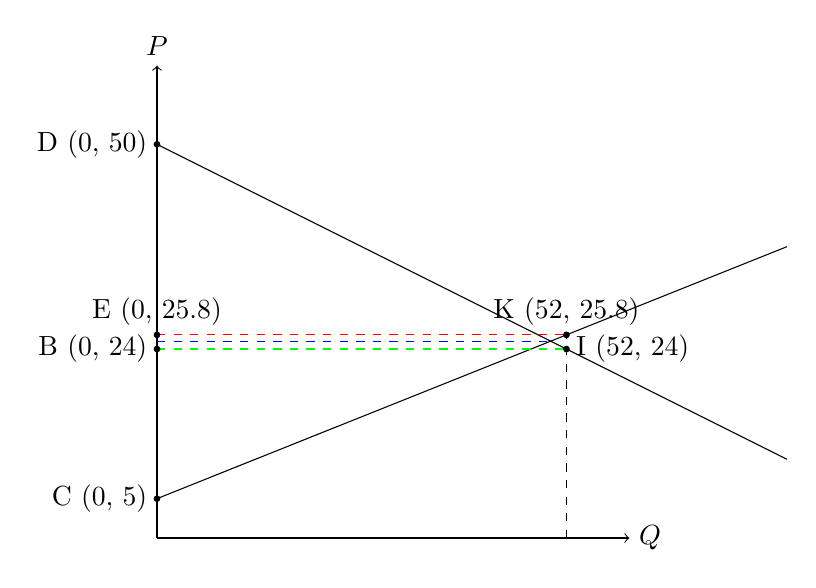
\begin{tikzpicture}
          \draw [->] (0,0) -- (6,0)node[right] {$Q$};
          \draw [->] (0,0) -- (0,6)node[above] {$P$};

          %\filldraw[fill=blue!20, scale = 0.1] (0,50) -- (52,24) -- (0, 24) -- cycle;
          %\filldraw[fill=green!20, scale = 0.1] (0,3.2) -- (52,24) -- (0, 24) -- cycle;

          \draw[scale = 0.1, domain=0:80, smooth, variable=\x, color=black]
          plot ({\x}, {50 - \x / 2});
          \draw[scale = 0.1, domain=0:80, smooth, variable=\x, color=black]
          plot ({\x}, {\x / 2.5 + 5});


          \draw [dashed, scale = 0.1, color=black] (52,0) -- (52, 25.8);
          \draw [dashed, scale = 0.1, color=green] (0, 24) -- (52, 24);
          \draw [dashed, scale = 0.1, color=red] (0, 25.8) -- (52, 25.8);
          \draw [dashed, scale = 0.1, color=blue] (0, 25) -- (50, 25);


          \filldraw[scale = 0.1, color=black] (52, 24) circle (10pt) node[anchor=west]{I (52, 24)};
          \filldraw[scale = 0.1, color=black] (52, 25.8) circle (10pt) node[anchor=south]{K (52, 25.8)};
          %\filldraw[scale = 0.1, color=black] (0, 3.2)  circle (10pt) node[anchor=west]{A (0, 3.2)};
          \filldraw[scale = 0.1, color=black] (0, 24)  circle (10pt) node[anchor=east]{B (0, 24)};
          \filldraw[scale = 0.1, color=black] (0, 5)  circle (10pt) node[anchor=east]{C (0, 5)};
          \filldraw[scale = 0.1, color=black] (0, 50)  circle (10pt) node[anchor=east]{D (0, 50)};          

          \filldraw[scale = 0.1, color=black] (0, 25.8)  circle (10pt) node[anchor=south]{E (0, 25.8)};          

        \end{tikzpicture}

        Mỗi bên được hưởng bao nhiêu trợ cấp? Số tiền trợ cấp mà chính phủ phải chi ra là bao
        nhiêu? \\
        khoản trợ cấp của bên mua là chênh lệch giữa giá cân bằng và giá sau trợ cấp nhân với lượng cầu tại giá trợ cấp tức là : \\
        $(25 - 24) * 52$ \\
        khoản trợ cấp của bên bán là chênh lệch giữa giá cân bằng và giá sau trợ cấp nhân với lượng cung tại giá trợ cấp tức là : \\
        $(25.8 - 25) * 52$ \\
        số tiền trợ cấp của chính phủ là tích của mức trợ cấp nhân với sản lượng \\
        $1.8 * 52$
        
\end{enumerate}


\section{Thị trường mỳ tôm có phương trình }
đường cung $Q_S = 30 + 2P$ và phương trình
đường cầu $Q_D = 180 - 3P$ (P tính theo nghìn đồng/kg, Q tính theo triệu kg).: \\
(P tính bằng nghìn đồng/kg, Q tính bằng triệu kg) \\

\begin{enumerate}[a.]
  \item Tìm giá và lượng cân bằng trên thị trường? \\
        $Q_S = 30 + 2P = Q_D = 180 - 3P \Rightarrow 5P = 150 \Rightarrow P = 30, Q = 90$
  \item Giả sử chính phủ đánh thuế 10 nghìn đồng trên mỗi kg sản phẩm mà người tiêu dùng
        mua. Xác định giá và lượng cân bằng sau thuế? Tính gánh nặng thuế đối với người tiêu
        dùng và người sản xuất, số tiền thuế mà chính phủ thu được là bao nhiêu? \\
        theo 6.2.2 thì khi thuế đánh vào người mua; "Đường cầu dịch
        chuyển xuống dưới  1 khoảng đúng bằng  mức thuế t" \\
        ta viết phương trình đường cầu cũ:  \\
        $Q_D = 180 - 3P$\\
        phương trình cầu sau thuế là \\
        $P + 10 = 60 - Q_D / 3$ với ý nghĩa là với lương hàng hóa nhu cũ thì cần thêm 10 đồng mới mua được \\
        $P = 60 - Q_D / 3 - 10 = 50 - Q_D / 3 \Rightarrow Q_D = 150 -3P$\\
        điểm cân bằng mới tính như sau\\
        $150 - 3P = 30 + 2P \Rightarrow 5P = 120 \Rightarrow P = 24, Q = 78$

        ta sẽ vẽ đồ thị để dễ nhìn hơn \\
        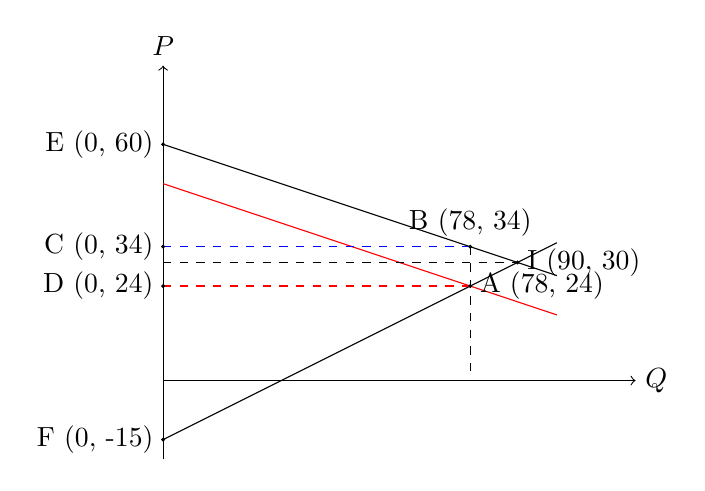
\begin{tikzpicture}
          \draw [->] (0,0) -- (6,0)node[right] {$Q$};
          \draw [->] (0,-1) -- (0,4)node[above] {$P$};

          \draw[scale = 0.05, domain=0:100, smooth, variable=\x, color=black]
          plot ({\x}, {\x / 2 - 15});
          \draw[scale = 0.05, domain=0:100, smooth, variable=\x, color=black]
          plot ({\x}, {60 - \x / 3 });
          \draw[scale = 0.05, domain=0:100, smooth, variable=\x, color=red]
          plot ({\x}, {50 - \x / 3});


          \draw [dashed, scale = 0.05, color=black] (0,30) -- (90,30);
          \draw [dashed, scale = 0.05, color=black] (78, 34) -- (78, 0);
          \draw [dashed, scale = 0.05, color=red] (0, 24) -- (78, 24);
          \draw [dashed, scale = 0.05, color=blue] (0, 34) -- (78, 34);


          \filldraw[scale = 0.05, color=black] (90, 30) circle (10pt) node[anchor=west]{I (90, 30)};
          \filldraw[scale = 0.05, color=black] (78, 24)  circle (10pt) node[anchor=west]{A (78, 24)};
          \filldraw[scale = 0.05, color=black] (78, 34)  circle (10pt) node[anchor=south]{B (78, 34)};
          \filldraw[scale = 0.05, color=black] (0, 34)  circle (10pt) node[anchor=east]{C (0, 34)};
          \filldraw[scale = 0.05, color=black] (0, 24)  circle (10pt) node[anchor=east]{D (0, 24)};
          \filldraw[scale = 0.05, color=black] (0, 60)  circle (10pt) node[anchor=east]{E (0, 60)};
          \filldraw[scale = 0.05, color=black] (0, -15)  circle (10pt) node[anchor=east]{F (0, -15)};
        \end{tikzpicture}

        Xác định giá và lượng cân bằng sau thuế? $P = 24, Q = 78$\\
        Tính gánh nặng thuế đối với người tiêu dùng và người sản xuất, số tiền thuế mà chính phủ thu được là bao nhiêu?\\
        với người tiêu dùng = 34 - 30 \\
        với người sản xuất = 30 - 24\\
        số tiền thuế = $S_{CBAD} = 78 * (34 - 24)$

  \item  Với mức thuế ở câu b, tính CS, PS, phần mất không do thuế gây ra là bao nhiêu?

        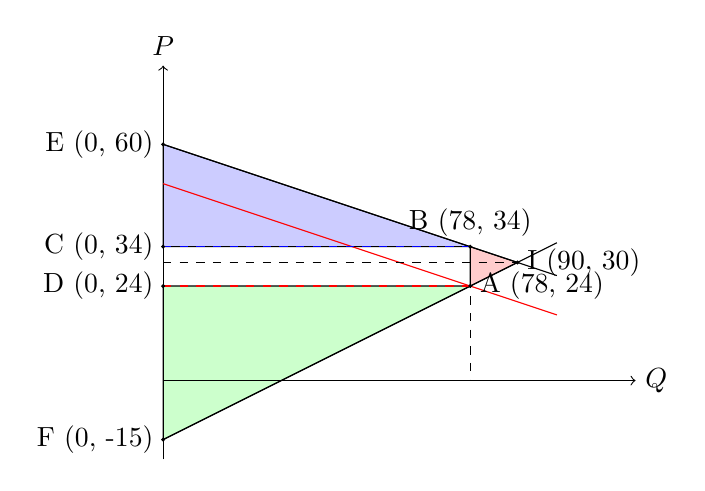
\begin{tikzpicture}


          \filldraw[fill=blue!20, scale = 0.05] (0,60) -- (78,34) -- (0, 34) -- cycle;
          \filldraw[fill=red!20, scale = 0.05] (78, 34) -- (90, 30) -- (78, 24) -- cycle;
          \filldraw[fill=green!20, scale = 0.05] (0 ,24) -- (78,24) -- (0, -15) -- cycle;

          \draw [->] (0,0) -- (6,0)node[right] {$Q$};
          \draw [->] (0,-1) -- (0,4)node[above] {$P$};

          \draw[scale = 0.05, domain=0:100, smooth, variable=\x, color=black]
          plot ({\x}, {\x / 2 - 15});
          \draw[scale = 0.05, domain=0:100, smooth, variable=\x, color=black]
          plot ({\x}, {60 - \x / 3 });
          \draw[scale = 0.05, domain=0:100, smooth, variable=\x, color=red]
          plot ({\x}, {50 - \x / 3});

          \draw [dashed, scale = 0.05, color=black] (0,30) -- (90,30);
          \draw [dashed, scale = 0.05, color=black] (78, 34) -- (78, 0);
          \draw [dashed, scale = 0.05, color=red] (0, 24) -- (78, 24);
          \draw [dashed, scale = 0.05, color=blue] (0, 34) -- (78, 34);


          \filldraw[scale = 0.05, color=black] (90, 30) circle (10pt) node[anchor=west]{I (90, 30)};
          \filldraw[scale = 0.05, color=black] (78, 24)  circle (10pt) node[anchor=west]{A (78, 24)};
          \filldraw[scale = 0.05, color=black] (78, 34)  circle (10pt) node[anchor=south]{B (78, 34)};
          \filldraw[scale = 0.05, color=black] (0, 34)  circle (10pt) node[anchor=east]{C (0, 34)};
          \filldraw[scale = 0.05, color=black] (0, 24)  circle (10pt) node[anchor=east]{D (0, 24)};
          \filldraw[scale = 0.05, color=black] (0, 60)  circle (10pt) node[anchor=east]{E (0, 60)};
          \filldraw[scale = 0.05, color=black] (0, -15)  circle (10pt) node[anchor=east]{F (0, -15)};
        \end{tikzpicture}

        CS = diện tích CEB = (60 - 34) * 78 / 2 \\
        PS = diện tích DFA = (24 - (-15)) * 78 / 2\\
        DWL = diện tích BAI = (34 - 24) * (90 - 78) / 2\\
        mọi người có thể ngạc nhiên về PS, tại sao lại có số -15, trong kinh tế, bán hàng giá âm chưa chắc đã là lỗ mà bán hàng giá dương chưa chắc đã là lãi

  \item Nếu chính phủ trợ cấp 10 nghìn đồng/kg mỳ tôm mà người tiêu dùng mua. Giá và sản
        lượng sẽ thay đổi như thế nào? Mỗi bên được hưởng bao nhiêu trợ cấp?

        khi nhận trợ cấp thì $P_S$ sẽ lớn hơn $P_D$ và $P_S - P_D = 10$ \\ 
        ta có các phương trình như sau\\
        $Q_S = 30 + 2P \Rightarrow P = Q_S / 2 - 15$ \\
        $Q_D = 180 - 3P \Rightarrow P = 60 - Q_D / 3$ \\
        $Q/ 2 - 15 - (60 - Q/ 3) = 10 \Rightarrow Q / 2 + Q / 3 = 15 + 60 + 10 = 85$ \\
        nhân 6 cho 2 vế \\
        $3 Q + 2 Q = 85 * 6 \Rightarrow Q = 102, P_S = 36, P_D = 26$

        

        ta sẽ vẽ đồ thị để dễ nhìn hơn \\
        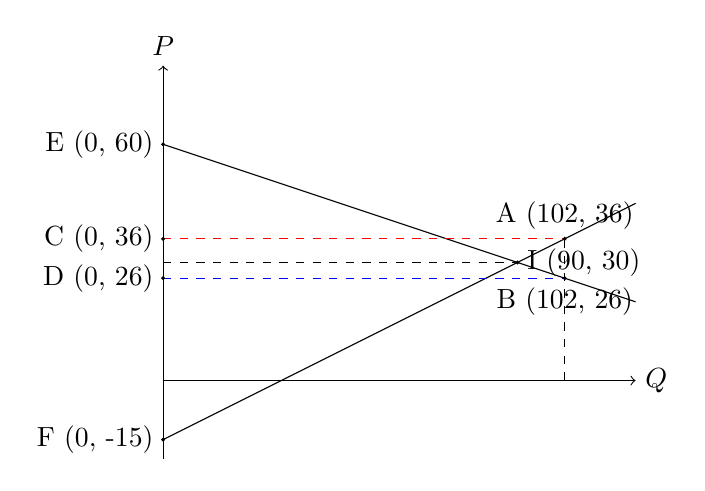
\begin{tikzpicture}
          \draw [->] (0,0) -- (6,0)node[right] {$Q$};
          \draw [->] (0,-1) -- (0,4)node[above] {$P$};

          \draw[scale = 0.05, domain=0:120, smooth, variable=\x, color=black]
          plot ({\x}, {\x / 2 - 15});
          \draw[scale = 0.05, domain=0:120, smooth, variable=\x, color=black]
          plot ({\x}, {60 - \x / 3 });
        %  \draw[scale = 0.05, domain=0:120, smooth, variable=\x, color=red]          plot ({\x}, {70 - \x / 3});


          \draw [dashed, scale = 0.05, color=black] (0,30) -- (90,30);
          \draw [dashed, scale = 0.05, color=black] (102, 0) -- (102, 36);
          \draw [dashed, scale = 0.05, color=red] (0, 36) -- (102, 36);
          \draw [dashed, scale = 0.05, color=blue] (0, 26) -- (102, 26);


          \filldraw[scale = 0.05, color=black] (90, 30) circle (10pt) node[anchor=west]{I (90, 30)};
          \filldraw[scale = 0.05, color=black] (102, 36)  circle (10pt) node[anchor=south]{A (102, 36)};
          \filldraw[scale = 0.05, color=black] (102, 26)  circle (10pt) node[anchor=north]{B (102, 26)};
          \filldraw[scale = 0.05, color=black] (0, 36)  circle (10pt) node[anchor=east]{C (0, 36)};
          \filldraw[scale = 0.05, color=black] (0, 26)  circle (10pt) node[anchor=east]{D (0, 26)};
          \filldraw[scale = 0.05, color=black] (0, 60)  circle (10pt) node[anchor=east]{E (0, 60)};
          \filldraw[scale = 0.05, color=black] (0, -15)  circle (10pt) node[anchor=east]{F (0, -15)};
        \end{tikzpicture}

        Mỗi bên được hưởng bao nhiêu trợ cấp?\\
        trợ cấp cho bên bán là khoảng thay đổi giữa giá cân bằng và giá bán khi được trợ cấp nhân với lượng hàng trên thị trường khi được trợ cấp\\
        $(36 - 30) * 102$ \\
        trợ cấp cho bên mua là khoảng thay đổi giữa giá cân bằng và giá mua khi được trợ cấp nhân với lượng hàng trên thị trường khi được trợ cấp\\
        $(30 - 26) * 102$ \\
        


\end{enumerate}

\section{ Hàm số cầu của táo hàng năm có dạng }
$ Q_D = 100 - 1/2P$ (P –1000 đồng/kg; Q-tấn). \\
Mùa thu hoạch táo năm trước là 80 tấn tại mọi mức giá. Năm
nay, thời tiết không thuận lợi nên lượng thu hoạch táo năm nay chỉ đạt 70 tấn tại mọi mức
giá (táo không thể tồn trữ)
\begin{enumerate}[a.]
  \item Xác định giá táo năm nay trên thị trường. Tính CS, PS tại mức giá này ?

        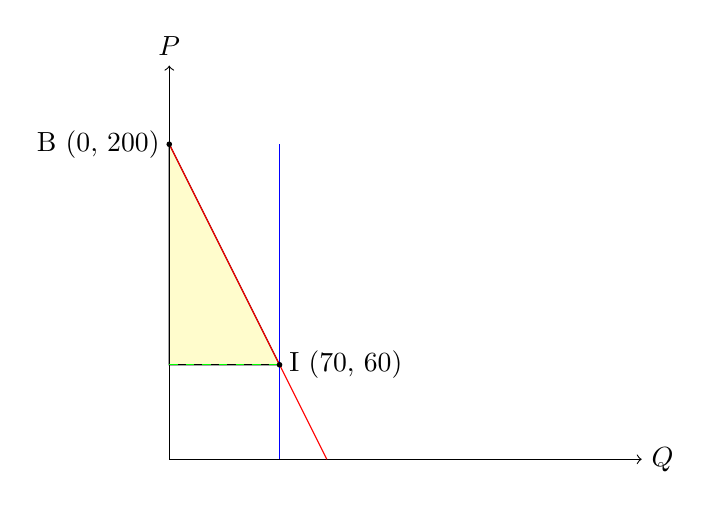
\begin{tikzpicture}
          \draw [->] (0,0) -- (6,0)node[right] {$Q$};
          \draw [->] (0,0) -- (0,5)node[above] {$P$};


          \filldraw[fill=yellow!20, scale = 0.02] (0,200) -- (70, 60) -- (0, 60) -- cycle;

          \draw[scale = 0.02, domain=0:100, smooth, variable=\x, color=red]
          plot ({\x}, {200 -  2 *\x   });

          \draw [dashed, scale = 0.02, color=green] (0,60) -- (70, 60);
          \draw [-, scale = 0.02, color=blue] (70, 200) -- (70, 0);
          %\draw [dashed, scale = 0.05, color=red] (0, 24) -- (78, 24);
          %\draw [dashed, scale = 0.05, color=blue] (0, 34) -- (78, 34);

          \filldraw[scale = 0.02, color=black] (70, 60) circle (40pt) node[anchor=west]{I (70, 60)};
          \filldraw[scale = 0.02, color=black] (0, 200)  circle (40pt) node[anchor=east]{B (0, 200)};

        \end{tikzpicture}

        thay Q = 70 vào phương trình cầu ta có P = 60 vậy giá là 60 \\
        CS là diện tích nằm trên giá và dưới đường cầu, \\
         vậy CS = (200 - 60) * 70 / 2\\
        do đường cung song song với trục tung nên chúng ta không tính được PS

  \item Tính hệ số co giãn của cầu tại mức giá này. Bạn có nhận xét gì về thu nhập của
        người trồng táo năm nay so với năm trước.

        ta viết lai phương trình đường cầu $ Q_D = 100 - 1/2P$ \\
        $P = 200 - 2Q_D$

         ta có công thức tính hệ số co giãn của cầu tại điểm như sau

         \[ E_{DP} = \frac{\%\Delta Q_D}{\%\Delta P} =
         \frac{\Delta Q_D}{\Delta P} \times \frac{P}{Q_D} = Q_D' \times \frac{P}{Q_D} \]

         $E_{DP} = -2 \times \frac{60}{70} = -1.714$\\
         giá trị tuyệt đối của $E_{DP}$ lớn hơn 1, do đó cầu co giãn theo giá 


  \item Để đảm bảo thu nhập cho người trồng táo chính phủ ấn định mức giá sàn năm nay
        là 70 nghìnđ/kg và cam kết hứa mua hết phần lúa dư thừa thì số tiền chính phủ phải
        chi ra là bao nhiêu?

        \begin{tikzpicture}
          \draw [->] (0,0) -- (6,0)node[right] {$Q$};
          \draw [->] (0,0) -- (0,5)node[above] {$P$};


          %\filldraw[fill=yellow!20, scale = 0.02] (0,200) -- (70, 60) -- (0, 60) -- cycle;

          \draw[scale = 0.02, domain=0:100, smooth, variable=\x, color=red]
          plot ({\x}, {200 -  2 *\x   });

          %\draw [dashed, scale = 0.02, color=violet] (0,60) -- (70, 60);
          \draw [-, scale = 0.02, color=blue] (70, 200) -- (70, 0);
          \draw [dashed, scale = 0.02, color=green] (0, 70) -- (70, 70);
          %\draw [dashed, scale = 0.05, color=blue] (0, 34) -- (78, 34);

          \filldraw[scale = 0.02, color=black] (70, 70) circle (40pt) node[anchor=west]{I (70, 70)};
          \filldraw[scale = 0.02, color=black] (0, 200)  circle (40pt) node[anchor=east]{B (0, 200)};
          \filldraw[scale = 0.02, color=black] (65, 70)  circle (40pt) node[anchor=north]{A (65, 70)};

        \end{tikzpicture}

        tại mức giá P = 70, giao của nó với đường cầu tại A(65, 70)\\
        điều đó có nghĩa là thị trường chỉ mua 65 tấn, còn dư 70 - 65 = 5 tấn\\
        chính phủ sẽ thu mua với giá 70 vậy số tiền chi ra là 70 * 5 = 350

  \item Nếu chính phủ đánh thuế mỗi kg táo mà người tiêu dùng mua là 5 nghìn đồng, thì
        giá cả cân bằng và sản lượng cân bằng thay đổi thế nào? Ai là người chịu thuế? Giải
        thích ?

        ở đây cung không đổi , ta có thể hiểu đó là đánh vào người mua, đường càu dịch chuyển chuyển xuống dưới
        1 khoảng đúng bằng
        mức thuế t theo như 6.2.2\\
        ta có phương trình cầu cũ $P = 200 - 2Q_D$ \\
        thuế đánh 5 nghìn đồng thì đường cầu mới sẽ là \\
        $P + 5 = 200 - 2Q_D$  ở đâu lượng cầu không đổi nhưng giá tăng thêm 5 đơn vị\\
        $P = 195 - 2Q_D$

        giá cân bằng sẽ là $P = 195 - 2 * 70 = 55$ vì sản lượng là không đổi


        \begin{tikzpicture}
          \draw [->] (0,0) -- (8,0)node[right] {$Q$};
          \draw [->] (0,0) -- (0,8)node[above] {$P$};


          %\filldraw[fill=yellow!20, scale = 0.02] (0,200) -- (70, 60) -- (0, 60) -- cycle;

          \draw[scale = 0.1, domain=60:100, smooth, variable=\x, color=black]
          plot ({\x}, {200 -  2 *\x   });

          \draw[scale = 0.1, domain=60:100, smooth, variable=\x, color=red]
          plot ({\x}, {195 -  2 *\x   });

          %\draw [dashed, scale = 0.02, color=violet] (0,60) -- (70, 60);
          \draw [-, scale = 0.1, color=blue] (70, 100) -- (70, 0);
          \draw [dashed, scale = 0.1, color=black] (0, 60) -- (70, 60);
          \draw [dashed, scale = 0.1, color=blue] (0, 55) -- (70, 55);

         \filldraw[scale = 0.1, color=black] (0, 60) circle (10pt) node[anchor=east]{P \& $P_D$};
         \filldraw[scale = 0.1, color=black] (0, 55)  circle (10pt) node[anchor=east]{$P_S$};
         % \filldraw[scale = 0.02, color=black] (65, 70)  circle (40pt) node[anchor=north]{A (65, 70)};

        \end{tikzpicture}

        chúng ta có thể nhìn thấy, sau khi đánh thuế, đường cầu dịch chuyển sang trái, do cung không đổi nên $P_S$ giảm xuống trong khi $P_D$ giữ nguyên, đo đó người bán đang bị đánh thuế\\
        điều này cũng thể hiện trong mục 6.2.3 Hệ số co giãn và sự phân chia 
        gánh nặng thuế

\end{enumerate}